\newpage
\section{集成学习}

\subsection{个体与集成}
集成学习(ensemble learning)通过构建并结合多个学习器来提
升性能

在一定条件下,随着集成分类器数目的增加,集成
的错误率将指数级下降,最终趋向于0


\subsection{Boosting}
先从初始训练集训练出一个基学习器,再根据基学习器的表现对训练
样本分布进行调整,使得先前基学习器做错的训练样本在后续受到更多关注,
然后基于调整后的样本分布来训练下一个基学习器;如此重复进行,直至基学
习器数目达到事先指定的值$T$ , 最终将这$T$ 个基学习器进行加权结合.

\begin{figure}[!htb]
    \centering
    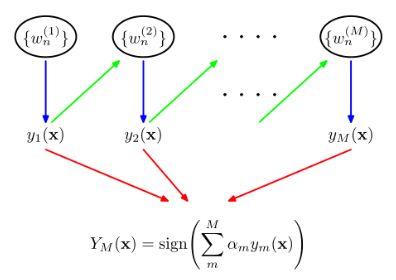
\includegraphics[width=0.309\textwidth]{pic/ML8/Boosting}
    \caption{Boosting}
\end{figure}

\subsubsection{Adaboost}
AdaBoost算 法 有 多 种 推 导 方 式. 跳过推导了. 

数据分布的学习: 重赋权法, 重采样法. 

重启动,避免训练过程过早停止

\subsection{Bagging与随机森林}
\subsubsection{Bagging}
Bagging是并行式集成学习方法最著名的代表. 

使用可重复采样采样出$T$ 个 含 $m$ 个训练样本的采样集,然后基于每个采样集训练出一个基学习器,再将这些基学习器进行结合.

结果通过投票法或比较置信度确认. 

训练一个bagging集成与直接使用基学习器的复杂度同阶. 

\subsubsection{随机森林}
随机森林(Random Forest,简称 RF)是 Bagging 的一个
扩展变体. RF 在以决策树为基学习器构建Bagging集成的基础上,进一步在
决策树的训练过程中引入了随机属性选择

\subsection{结合策略}
学习器结合可能会从三个方面带来好处: 
\begin{enumerate}
    \item 从统计
    的方面来看,由于学习任务的假设空间往往很大,可能有多个假设在训练集上
    达到同等性能,此时若使用单学习器可能因误选而导致泛化性能不佳,结合多
    个学习器则会减小这一风险
    \item 从计算的方面来看,学习算法往往会陷入局
    部极小,有的局部极小点所对应的泛化性能可能很糟糕,而通过多次运行之后
    进行结合,可降低陷入糟糕局部极小点的风险
    \item 从表示的方面来看,某些
    学习任务的真实假设可能不在当前学习算法所考虑的假设空间中,此时若使用
    单学习器则肯定无效,而通过结合多个学习器,由于相应的假设空间有所扩大,
    有可能学得更好的近似
\end{enumerate}


\subsubsection{平均法}
对数值型输出$h_i(\bx)\in\R$, 最常见的结合策略是使用平均法(averaging).
\begin{itemize}
    \item 简单平均法(simple averaging)
    \begin{align*}
        H(\bx)=\frac{1}{T}\sum_{i=1}^T h_i(\bx)
    \end{align*}
    \item 加权平均法(weighted averaging)
    \begin{align*}
        H(\bx)=\sum_{i=1}^Tw_ih_i(\bx)
    \end{align*}
    $w_i$  是个 体 学 习 器 $h_i$ 的权重, 通常要求 $w_i\ge 0, \displaystyle \sum_{i=1}^Tw_i=1$
\end{itemize}
\subsubsection{投票法}
\begin{itemize}
    \item 绝对多数投票法(majority voting)
    \subitem 若某标记得票过半数,则预测为该标记;否则拒绝预测.
    \item 相对多数投票法(plurality voting)
    \subitem 预测为得票最多的标记, 若同时有多个标记获最高票,则从中随机选取
    一个.
    \item  加权 投 票 法 (weighted voting)
    \subitem 与加权平均法类似
\end{itemize}
\subsubsection{学习法}
通过另一个学习器来进行结合. Stacking是学习法的典型代表, 多响应线性回归(MLR)作为次级学习器的学习算法, 效果较好. 


贝叶斯模型平均(Bayes Model Averaging,简 称 BMA)基于后验概率来为
不 同 模 型 赋 予 权 重 ,可 视 为 加 权 平 均 法 的 一 种 特 殊 实 现 . 


\subsection{多样性}
\subsubsection{误差-分歧分解}
定 义 个体学 习 器 $h_i$ 与集成学习器 $H$的分歧为 
\begin{align*}
    A(h_i|\bx)=(h_i(\bx)-H(\bx))^2
\end{align*}
经过一系列对回归问题的推导后, 
\begin{align*}
    E=\bar{E}-\bar{A}
\end{align*}
$\bar{E}$表示 个 体 学 习 器 泛化误差的加权均值, $\bar{A}$表示个体学习器的加权分歧值

这个漂亮的式子显示:个体学习器精确性越高、多样性越大,则集成
效果越好。称为误差-分歧分解


\subsubsection{多样性度量}
多样性度量(diversity measure)是用于估算个体学习器的多样化程度. 

常见的多样性度量:
\begin{itemize}
    \item 不合度量(Disagreement Measure)
    \item 相关系数(Correlation Coefficient)
    \item $Q$-统计量(Q-Statistic)
    \item $\kappa$-统计量(Kappa-Statistic)
\end{itemize}
\subsubsection{多样性增强}
常见的增强个体学习器的多样性的方法:
\begin{itemize}
    \item 数据样本扰动
    \item 输入属性扰动
    \item 输出表示扰动
    \item 算法参数扰动
\end{itemize}